% -*- Mode:TeX -*-
% LaTeX template for CinC papers                   v 1.1a 22 August 2010
%
% To use this template successfully, you must have downloaded and unpacked:
%       http://www.cinc.org/authors_kit/papers/latex.tar.gz
% or the same package in zip format:
%       http://www.cinc.org/authors_kit/papers/latex.zip
% See the README included in this package for instructions.
%
% If you have questions, comments or suggestions about this file, please
% send me a note!  George Moody (george@mit.edu)
%
\documentclass[twocolumn]{cinc}
\usepackage{graphicx}
%\usepackage{subcaption}
\newcommand{\mapthreed}{\textit{map3d }}
\begin{document}

% Keep the title short enough to fit on a single line if possible.
% Don't end it with a full stop (period).  Don't use ALL CAPS.
\title{Electrocardiographic Comparison of Dobutamine and BRUCE Cardiac \\ Stress Testing With High Resolution Mapping in Experimental Models}

% Both authors and affiliations go in the \author{ ... } block.
% List initials and surnames of authors, no full stops (periods),
%  titles, or degrees.
% Don't use ALL CAPS, and don't use ``and'' before the name of the
%  last author.
% Leave an empty line between authors and affiliations.
% List affiliations, city, [state or province,] country only
%  (no street addresses or postcodes).
% If there are multiple affiliations, use superscript numerals to associate
%  each author with his or her affiliations, as in the example below.

\author { Brian Zenger$^{1,2,3,4}$, Wilson W Good$^{1,2,3}$, Jake Bergquist$^{1,2,3}$ Jess D Tate$^{1,2,3}$, Vikas Sharma$^{4}$, \\Rob S MacLeod$^{1,2,3}$\\
\ \\ % leave an empty line between authors and affiliation
$^1$ Scientific Computing and Imaging Institute, University of Utah, SLC, UT, USA \\
$^2$  Nora Eccles Cardiovascular Research and Training Institute, University of Utah, SLC, UT, USA \\
$^3$ Department of Biomedical Engineering, University of Utah, SLC, UT, USA \\
$^4$ School of Medicine, University of Utah, SLC, UT, USA }

\maketitle

% LaTeX inserts the ``Abstract'' heading in the proper style and
% sets the text of the abstract in italics as required.
\begin{abstract}

    Clinical tests to detect acute myocardial ischemia induce transient
    cardiac stress by means of exercise or pharmaceutical stimulation and
    measure electrical changes of the heart on the body surface via an
    electrocardiogram (ECG).  Such tests assume that both stress mechanisms
    induce identical--—or at least similar—--forms of ischemia. However,
    results of these tests have been known to contradict each other. To
    improve electrocardiographic detection of myocardial ischemia,
    we must study how varied stressing agents (pharmacological or paced
    stressors) change electrocardiographic signatures. We simultaneously measured electrical recordings within the
    myocardium, on the epicardial surface, and on the body surface. We then
    induced acute, controlled ischemia and monitored the electrical
    response. To create the hemodynamic substrate for ischemia, we
    applied a constant hydraulic occlusion to the left anterior
    descending coronary artery. We varied the ischemic stress with
    two commonly used clinical protocols, the BRUCE and dobutamine stress
    tests. Each episode lasted 15 minutes with stepwise increase in pacing
    rate or pharmacological infusion rate every 3 minutes. Preliminary
    qualitative results suggest significant differences in the recorded
    electrical signal between pacing and pharmacological stress
    mechanisms. Differences include the location and volume of ischemia and
    its temporal development throughout a stress episode. These
    results, and the experimental means used to
    obtain them, are a significant breakthrough in the field with
    simultaneous, high density electrical recordings within the myocardium and on the heart and
    torso surfaces.

\end{abstract}
% LaTeX inserts the extra space here automatically.

\section{Introduction}
% Section numbering is automatic.  The examples on the next page
% illustrate how to make subsections.

% [|<Note that the spacing \cite commands is important.
% `globally. \cite{Roth2015}' creates a gap while
% `globally.\cite{Roth2015}' produces none.  I like the latter convention
% but the main thing is to be consistent.]

Ischemic heart disease is one of the most common heart pathologies,
effecting over 8 million people globally. \cite{Roth2015} Myocardial
ischemia occurs when the demand for nutrients and perfusion by the heart
outweighs the available supply. This imbalance recreates a supply-demand
mismatch that can lead to devastating long term consequences including
increased risk for myocardial infarction, cardiac arrhythmia, and sudden
cardiac death.\cite{Roth2015} For decades the electrocardiogram (ECG) has
been the primary acute detection method for myocardial
ischemia. \cite{McCarthy1990} However, current electrocardiographic
methods used to detect myocardial ischemia are mediocre at best, with
reported sensitivity and specificity ranging from 50-72\% and 69-90\%,
respectively. \cite{Akkerhuis2011} This poor performance indicates
that many patients are released from clinical care unaware of their
potentially life-threatening condition while others receive care they do
not need. Improvements in the electrical detection of myocardial ischemia
must be made to ensure patients and physicians can be confident in
diagnosing and treating myocardial ischemia early to prevent potentially
fatal long term consequences.

One possible source of this poor ECG-based performance may originate
from different cardiac stressing mechanisms. Clinical tests induce
transient cardiac stress by means of exercise or pharmaceutical stimulation
and measure electrical changes of the heart on the body surface via an
ECG. Such tests assume that both mechanisms induce identical, or at least
similar, forms of ischemia. However, no definitive experiments have been
reported that assess the electrical effects produced during
different stressing mechanisms. This lack of definitive study 
substantiates a controlled examination of these different stressing methods.

To date, no experimental model has provided accurate and comprehensive sampling of
electrical signals from controlled ischemia within the myocardial
tissue, on the heart surface, and on the body surface. A model with all of these
components is necessary to understand how the ischemic regions develop
within the heart, and how they manifest on the body surface. For this
study, our goal was to test the differences in myocardial ischemia
development under two
clinical cardiac stressing mechanisms, pacing the heart according to the BRUCE protocol and continuous
dobutamine infusion.


%
%\begin{figure}[h]
%%\centering
%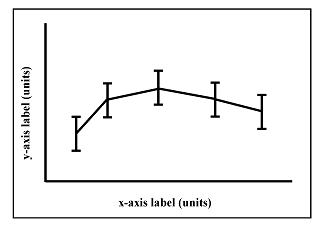
\includegraphics[width=7.9cm]{graph.png}
%\caption{Put the figure legend here, clearly describing the figure.}
%\label{FIGURA1}
%\end{figure}

%Always leave a line space after a figure legend. Avoid background colors as they can make printed figures hard to read.

\section{Methods}

\subsection{Animal Model} 

Swine and canine animal models were selected for this experimental
preparation because of their similar cardiac
anatomy, electrical system, and vascular structure to humans. The animals
of each species were 25--35 kg in weight and 8 months to
several years of age. The animals were purpose bred for the use
in experimental research and all studies were approved by the
Institutional Animal Care and Use Committee at the University of Utah and
conformed to the Guide for Care and Use of Laboratory Animals. After 12
hours of fasting, the animals were sedated using an intravenous propofol
bolus of 5--8~mg/kg in canines or a mixture of Telazol
(4.4~mg/kg), Ketamine (2.2~mg/kg), and Xylazine (2.2~mg/kg) in swine and then intubated. Once intubated,
isoflurane gas (1-5\%) was used for anesthesia. At the end of the
experiment animals were euthanized while under general anesthesia, with
intravenous Beuthanasia 1~ml/10~kg. The heart was then removed for further
evaluation.

\subsection{Surgical Procedure}

Following sedation, a sternotomy was performed to expose the thoracic
cavity. The pericardium was opened and the heart was suspended in a
pericardial cradle. Following exposure, a portion of the left anterior
descending coronary artery (LAD) was dissected and a calibrated hydraulic
occluder (Access Technologies, Skokie, IL, USA) was placed around the
dissected portion. An atrial pacing clip was then
placed on the appendage of the right atrium. Following placement of
the electrical recording equipment (described below), the pericardium was
sutured closed and the sternum was wired and sutured together. To limit air
within the volume conductor, chest tubes were tunneled into the
mediastinal, pleural, and pericardial cavities and held under constant
vacuum suction. The outer layers of dermis were sutured closed and checked
for potential separations. Standard laboratory markers were measured and
recorded throughout the experiment including blood pH,${\rm PaCO_2}$ , oxygen saturation,
temperature, and blood pressure.

\subsection{Electrical Recording Equipment}

\subsubsection{Electrode Arrays}

Electrical recording equipment was all custom build at the Nora Eccles
Treadwell Cardiovascular Research and Training Institute (CVRTI). The
electrical signals within the myocardium were measured using transmural
plunge needle arrays with 10 electrodes spaced 1.6 or 1.0 mm apart for left
and right ventricular needles, respectively. For these experiments,
12--25 needles were placed in the assumed perfusion bed of the LAD and concentrated on the anterior surface of the heart. The
epicardial potentials were measured using a 247-electrode sock array with
evenly spaced electrodes stitched into a nylon stocking material. The
distance between sock electrodes was approximately 10~mm. The torso surface
electrodes were in linear strips of 12 electrodes evenly spaced at 3~cm
apart. Each electrode had an 11~mm diameter Ag-AgCl sensor embedded in
an epoxy housing with a 2~mm deep gel cavity. The number of strips applied
to the torso surface varied between 6--10 
(72--120 total electrodes) depending on the body surface area
accessible for each animal.

\subsubsection{Data Acquisition}

The potentials from the sock, needle, and torso surface electrodes were
recorded using a custom acquisition system. This system could record
simultaneously from 1024~channels at 1~kHz sampling rate and 12~bit
resolution. Briefly, the acquisition system consisted of multiplexers,
interface circuitry, and a personal computer (PC) hosting a custom program
written in Labview (National Instruments, Austin, TX, USA) that managed the
hardware and allowed continuous signal acquisition. A bandpass filter with
cutoff frequencies at 0.03 and 500~Hz avoided both DC potentials and
aliasing.  Wilson's central terminal leads were used as the remote
reference for all the unipolar signals recorded from the sock, needles,
and torso surface electrodes. Prior to each experiment, calibration signals
were recorded for each channel.


\subsection{Ischemia Intervention Protocols}

During each experiment, several transient ischemic interventions
could be induced. Each of these interventions lasted between 8--15
minutes and were followed by a 30-minute rest period. The BRUCE exercise
stress was simulated by increasing paced heart rate a set amount above
resting heart rate every three minutes for fifteen minutes. This increase
in heart rate was predetermined from average increased heart rates
during BRUCE stress protocols reported in the
literature. \cite{Okin1986a} The occlusion percentage was fixed throughout
the stress interval. The intervention was terminated with the
presence of a sequence of three or more premature ventricular
contractions. During the dobutamine stress protocol, the
animal was continuously infused at a a sequence of doses,
each for three minutes. Dosages followed the standard clinical
dobutamine stress testing protocols \cite{Secknus1997} and the
intervention again lasted 15 minutes or until a sequence of three
premature ventricular contractions occurred.

\subsubsection{Image Acquisition and Segmentation}

After each experiment, the intact torso was imaged with a clinical
3-Tesla MRI (Seimens Medical) for gross anatomy and electrode
positions. Following the full torso scan, the heart was excised and scanned
with a 7-Tesla MRI scanner (Bruker BIOSPEC 70/30, Billerica, MA) using FISP
(Fast Imaging with Steady-state Precession) and FLASH (Fast Low Angle Shot)
imaging sequences. To visualize fiber orientation in each heart, a
diffusion-weighted MRI sequence was also performed. Capitalizing on the combined advantages of both FISP (consistent
volume boundaries) and FLASH sequences (high internal contrast), we
produced geometric segmentations of cardiac tissue,
blood, and transmural plunge needle geometries using the Seg3D open-source
software package (https://www.sci.utah.edu/software/seg3d).

\subsection{Geometric Registration}

%\subsubsection{Landmark Point Recordings}

At the conclusion of each experiment, the locations of the linear torso
surface electrode strips, preselected sock electrodes, and
plunge needle insertion sites on the cardiac surface were digitally
recorded using a Microscribe three-dimensional digitizer (Solution
Technologies, Oella, MD, USA). In addition, landmark sites including the
location of the occlusion site, major epicardial
coronary arteries, and the outline of the myocardial shape were also
captured using the digitizer. Once the locations of the plunge needles were
recorded, they were replaced with plastic spacers.


\subsection{Signal Processing and Data Visualization}

The electrical signals recorded during the study were processed in
``Preprocessing Framework for Electrograms Intermittently Fiducialized from
Experimental Recordings'' (PFEIFER) program an open-source MATLAB-based
signal processing platform designed to process bioelectric signals acquired
from cardiac experiments. \cite{Rodenhauser2018} Using
PFEIFER, we were able to calibrate, baseline correct, filter, and mark
specific time instances within cardiac signals for analysis.

Finally, the processed experimental signals were mapped to the
identified electrode locations within the heart, on the epicardial surface
of the heart, and on the torso surface. Full experimental model datasets
were then visualized using \mapthreed
(https://www.sci.utah.edu/software/map3d) or SCIRun
(https://www.sci.utah.edu/software/scirun) open-source software
packages which provided for
extensive spatial exploration of the results.

\section{Results}

With this experimental preparation, we were
able to simultaneously record from all three aforementioned regions with
high resolution and adequate coverage. Ischemic control was achieved and four transient episodes of
ischemia were induced for each animal.

Figure \ref{fig:myo} shows one result to illustrate
the differences in the region of ischemia created during the BRUCE and
Dobutamine stress tests. During peak ischemic stress, the region
identified as ischemic based on elevated ST\%40 potentials was
larger following the dobutamine protocol than in the BRUCE protocol. 
Figure \ref{fig:epitorso} shows how these features also
propagated to the epicardial and body surfaces with the expected loss of
localization.


\begin{figure}
	\centering
	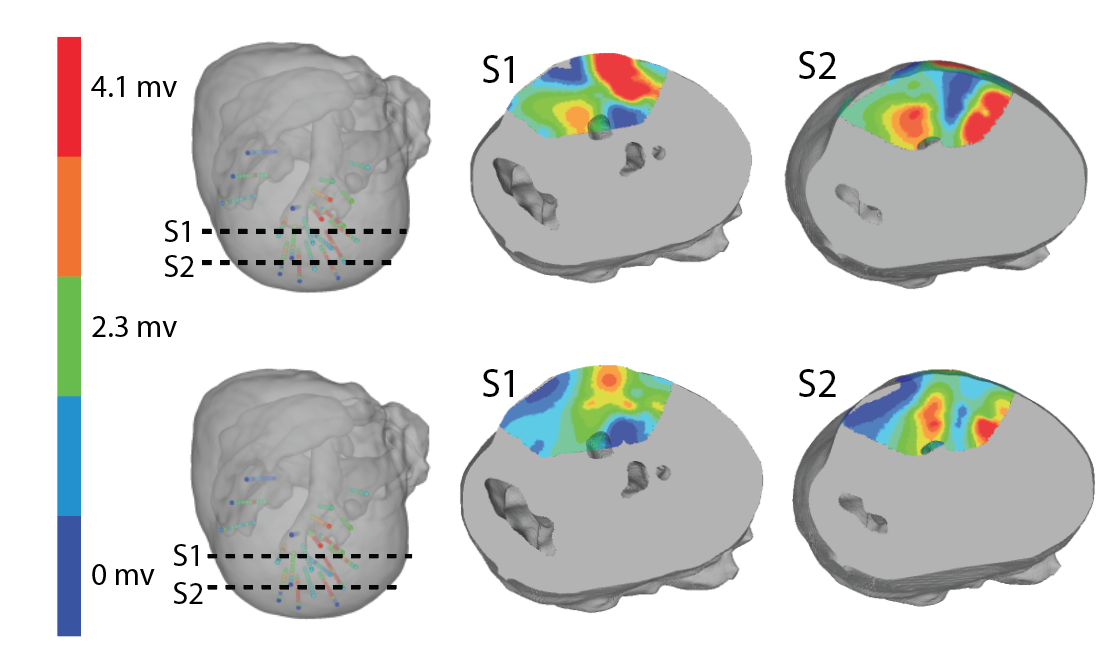
\includegraphics[width = .45\textwidth]{../Figures/1.png}
	
	\caption{Regions of ischemia detected within the myocardium. ST\%40 values are indicated by the color, as shown in the scale bar. The dashed lines indicate the slice
          levels captured in the adjacent projections. Row 1: Bruce
          protocol. Row 2: Dobutamine Protocol. The superior edge of each
          slice corresponds to the anterior surface in the leftmost
          column.}
	\label{fig:myo}
\end{figure}

\begin{figure}
	\centering
	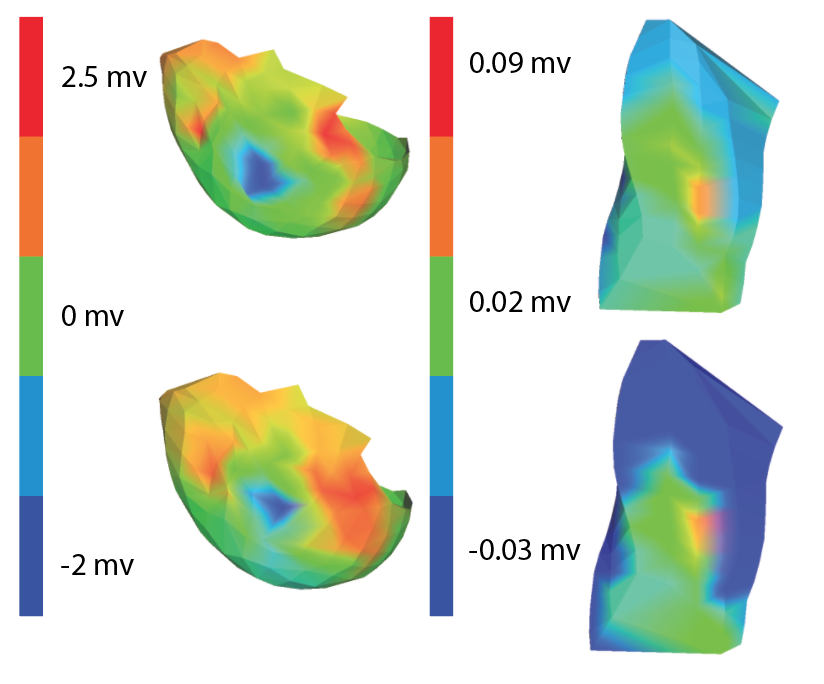
\includegraphics[width = .45\textwidth]{../Figures/2.png}

	\caption{Regions of ischemia detected on the epicardial surface and
          the torso surface. Again, color indicates
          amplitude of the local ST\%40 values Row 1: Epicardial and
          Torso measurements from a Bruce Protocol. Row 2: Epicardial and
          Torso Measurements from a dobutamine protocol.  Results are
          from the same cases as in Figure~\ref{fig:myo}}
	\label{fig:epitorso}
\end{figure}

\section{Discussion}

In this study, we proposed a novel experimental preparation to
characterize and understand the electrical signals of myocardial ischemia
within the heart and on the epicardial and body surfaces. In specific, we
tested the hypothesis that different clinical cardiac stress tests cause
different electrical signatures detectable on the body surface. Our results
show that  the BRUCE and dobutamine
stress tests produce different amounts and spatial distributions of
ischemia with comparable heart rates. The largest differences were visible within the myocardium,
as shown in the number and locations of extrema in Figure~\ref{fig:myo}.
Epicardial and torso surface differences were also visible but limited to
amplitudes of shared features. The dobutamine stress tests produced body
surface signals with significant amounts of depression, while the BRUCE
protocols produced only relatively mild depression.

These findings suggest different means of
stressing the heart require unique diagnostic criteria to detect and
monitor myocardial ischemia. This finding underscores a recurring theme
that the process of ischemia detection and development is more complicated
than conventional explanations have indicated. Our previous results have
already demonstrated that non-transmural ischemia arises from multiple
regions with the myocardium and shows complex spatio-temporal
progression.\cite{Aras2016}

Another important breakthrough in this study was the simultaneous
recordings from within the heart, on the heart surface, and on the body
surface during a controlled ischemic intervention. To date, we know of no
published results documenting such high resolution with a similar protocol. The datasets used
in this study will be ideal test datasets for other methods of detecting
ischemia, including electrocardiographic imaging. The high resolution,
ischemic control, and simultaneous recordings in multiple region make these
datasets extremely valuable to the community at large.

This project was limited by the small number of
experiments performed so far. This
study was also limited in direct clinical translation because of the
animal torso shape and other anatomical features. Future directions of this
project will include more experiments performed
with both stress protocols.


\balance


\section*{Acknowledgements}  
% This section is not numbered.
% 
Support for this research comes from the NIH NIGMS Center for Integrative
Biomedical Computing (www.sci.utah.edu/cibc), NIH NIGMS grant
no. P41GM103545 and the Nora Eccles Treadwell Foundation for Cardiovascular
Research.


% LateX generates the ``References'' heading automatically and switches
% to 9 point type for the bibliography.  If you use BibTeX (recommended),
% follow the examples in the sample 'refs.bib' file to enter your references,
% and leave the following line unchanged.
\bibliography{library.bib}
\bibliographystyle{cinc}

% If you don't use BibTeX, comment out or remove the previous line, and
% uncomment the following line and the ``}\end{bibliography}'' line below:

% LaTeX inserts the ``Address for correspondence'' heading.
\begin{correspondence}
Brian Zenger\\
72 Central Campus Dr, Salt Lake City, UT 84112\\
zenger@sci.utah.edu
\end{correspondence}

%\end{document}


% % Remove the '%' from the previous line before formatting the final
% % version of your paper
% 
% \clearpage
% \setcounter{section}{-1}
% 
% \section{Instructions for preparing your paper}
% 
% \subsection{This document}
% 
% Please save this document and use the outline on the first page to
% prepare your paper.
% 
% Before formatting your paper, remove these
% instructions by uncommenting the \verb+\end{document}+ line that you
% will find in this document a few lines above this paragraph.
% 
% \subsection{Paper length}
% 
% Please limit your paper to no more than four pages.
% 
% \subsection{LaTeX formatting}
% 
% In order to use this template to create a paper in proper CinC
% style, you will also need to have the CinC LaTeX macros, which
% can be downloaded from http://www.cinc.org/authors\_kit/ in either
% .tar.gz or .zip format.  These files include instructions on
% how to use them, together with complete example papers
% illustrating how to include equations, figures, tables, and
% references.
% 
% \subsection{Title}
% 
% Avoid abbreviations and keep to one or two lines. Remember that the
% title should be easily understood when cited as a reference in another
% publication.
% 
% \balance % equalize column lengths -- see comments on final page below
% 
% \subsection{Section numbering}
% 
% Number your sections as illustrated, \emph{starting with 1.}
% % LaTeX does this automatically.
% 
% 
% \subsection{Tables and figures}
% 
% Tables and figures can fit across both columns if necessary.  Captions go
% above tables, but beneath figures.
% 
% 
% 
% 
% \subsection{Citations and references}
% 
% All references should be included in the text in square brackets in
% their order of appearance, e.g. [1] [1,2] [1--4]. In the reference list
% use the Vancouver style (see BMJ 1991;302:338--41 or New Engl J Med
% 1991;324:424--8).
% 
% References to Computers in Cardiology proceedings should now include
% the volume number. For volumes before 1997, set out as for book
% chapters giving publisher and place of publication, noting that the
% publisher changed from IEEE Computer Society Press to IEEE in 1995.
% 
% There are (at least) two ways to prepare references.  We recommend
% that you use BibTeX if you can, since it automatically numbers your
% citations and generates a properly sorted reference list in
% CinC format, complete with a section heading.
% 
% If you do not use BibTeX, prepare your list of references following
% the commented-out examples on the first page of this document.
% 
% 
% \subsection{Final page}
% 
% The text on the final page should be arranged so that both columns
% are approximately the same height.   Insert \verb+\balance+ anywhere
% within the first column, and LaTeX will
% even out the columns automatically.
% 
% 
% \subsection{End of instructions}
% 
% \emph{All of section 0 should be deleted before you format the
% final version of your paper.}
% 
\end{document}
